\section{Performance Evaluation} \label{performance}
The extension's performance goals are to provide our security guarantees without being a detriment to the end user's browsing experience. To this end, we take several timestamps throughout our code's execution. These were recorded using the Performance Web API. Note that while this API normally reports values as doubles, due to recent security threats, such as Spectre~\cite{DBLP:journals/corr/abs-1801-01203}, several browser developers have implemented countermeasures by reducing the precision of the DOMHighResTimeStamp resolution~\cite{reducetimeprecision,resolutionconsiderations}. In particular, Firefox reports these values as integer milliseconds. For our tests, we re-enabled higher precision values.

While our extension's functionality only applies at the network level, there is potential slowdown at the DOM processing level due to the optimization techniques the browser applies throughout several levels of the web page load pipeline. \autoref{fig:navigationtiming} shows the different timestamps provided by the Navigation Timing API~\cite{navigationtiming}, as well as a high-level description of the browser processing model. Since our filter listens on the onBeforeRequest event, none of the previous steps before Request are affected. In this section, we refer to the difference in time between responseEnd and requestStart as the "network filter time".

\begin{figure}[h]
 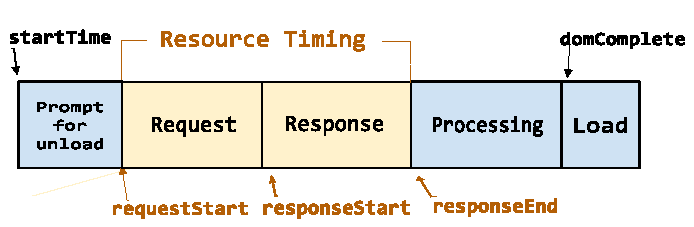
\includegraphics[scale=0.65]{img/timestamp-diagram-edited.pdf}
 \caption{The Navigation Timing API's timestamps\protect\footnotemark}
 \label{fig:navigationtiming}
 \end{figure}


\subsection{Top websites load times} \label{top_sites}

We first report our extension's impact on top website load times,
representing the expected behaviour of an user's average web browsing
experience. For these tests, we first took the top 500 websites as
reported by Moz.com~\cite{top500}. For each website, we loaded it 25
times (with a 25 second timeout) and recorded the following values:
requestStart, responseEnd, domComplete, and decodedBodySize. From the
initial 500, we only report values for 441 of them. The other 59 had
consistent issues with timeouts, insecure certificates, and network
errors. For our setup, we used a headless version of Firefox 69.0, and
Selenium WebDriver for NodeJS, with GeckoDriver. All experiments were
run on one machine with an Intel Xeon CPU E5-2407 2.40GHz processor,
32 GB DRAM, and our university's 1GiB connection. We ran four test
suites:

\begin{enumerate}
	\item No extension cold cache: Firefox is loaded without the extension installed and the web driver is re-instantiated for every page load.
	\item Extension cold cache: As in 1), but Firefox is loaded with the extension installed.
	\item No extension warm cache: Firefox is loaded without the extension installed and the same web driver is used for the page's 25 loads.
	\item Extension warm cache: As in 3), but Firefox is launched with the extension installed.
\end{enumerate}

\footnotetext{This image was taken from the w3 spec: \url{https://www.w3.org/TR/navigation-timing-2/}}

For each set of tests, we reduced the recorded values to two comparisons: network filter (responseEnd - requestStart), and page ready (domComplete - responseStart). The first analyzes the time spent by the network filter, while the second determines the time spent until the whole document has loaded. We calculate the medians for each website for each of these measures as well as the decodedByteSize.

\begin{figure}[h]
	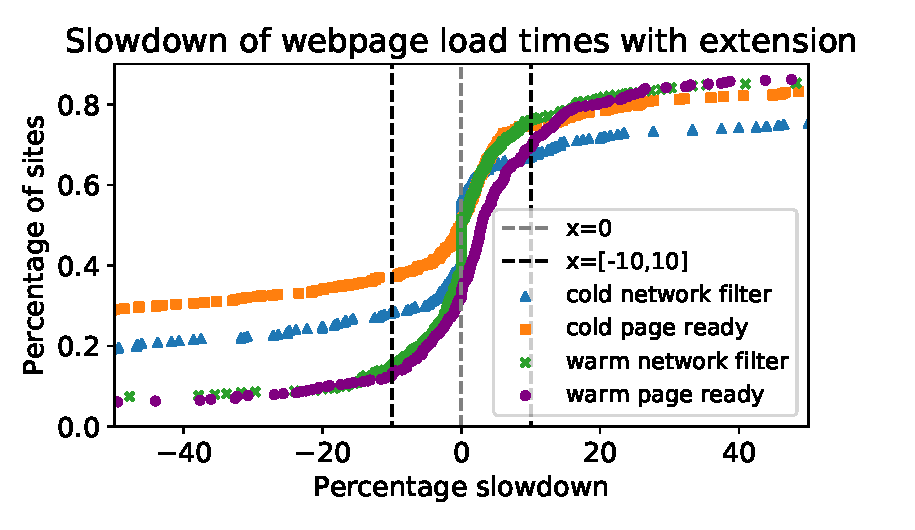
\includegraphics[scale=0.5]{results/extension_slowdown_overall_small.pdf}
	\caption{Cumulative distribution of relative percentage slowdown with extension installed for top sites.}
	\label{fig:overall_slowdown}
\end{figure}

We compare the load times with and without the extension running by calculating the relative slowdown with the extension installed according to the following formula:

\begin{equation*}
100*\frac{\tilde{x}_{with}-\tilde{x}_{without}}{\tilde{x}_{without}}
\end{equation*}
\\
where $\tilde{x}$ is the median with/without the extension running.

Figure ~\ref{fig:overall_slowdown} shows the computed results. The graph shows a slowdown of less than 10\% for 72.6\% of sites, and less than 50\% for 82\% of sites when the extension is running. Note that these values are recorded as percentages, and while some are as high as 50\%, the absolute values are in 77\% of cases less than a second. This overhead should not alter the user's experience significantly. The slowdown increases by at most 5\% when we take caching into account. This is likely because the network filter causes the browser to use less caching, especially for the DOM component, as it might have to process it from scratch every time. While it may seem counter-intuitive that some pages have shorter loading times without the extension, there are several variables at play that can affect these measurements (local network, server-side load, internal scheduling, etc). We manually checked the websites for which values were higher than |40\%| and verified that our extension did not change the page's contents, a possible cause for faster load times. We also checked the timings for the page as reported by the browser and noted a high variance even within small time windows. The time spent by our verification function was less than 10ms for 87.6\% of sites (\autoref{fig:verification_time_string_length}). This corroborates our findings that the slowdown is mostly negligible.

\iffalse
\begin{figure}[h]
	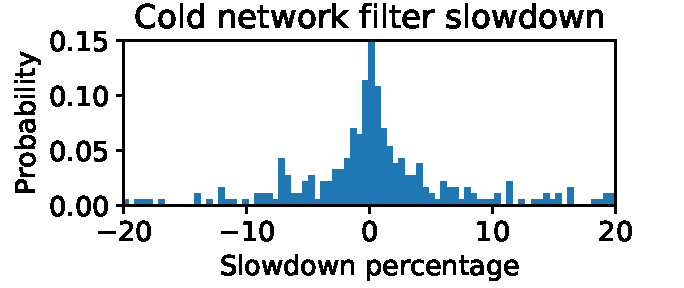
\includegraphics[scale=0.5]{results/density_histogram_filter_slowdown_small.pdf}
	\caption{Density histogram of network filter slowdown for top sites.}
	\label{fig:histogram_slowdown}
\end{figure}


Figure ~\ref{fig:histogram_slowdown} shows a closer look at the distribution for the cold network filter slowdown on the top sites (same values as in \autoref{fig:overall_slowdown}). For this component, 87.6\% of the slowdown values are less than 10\%.
\fi

\begin{figure}[h]
	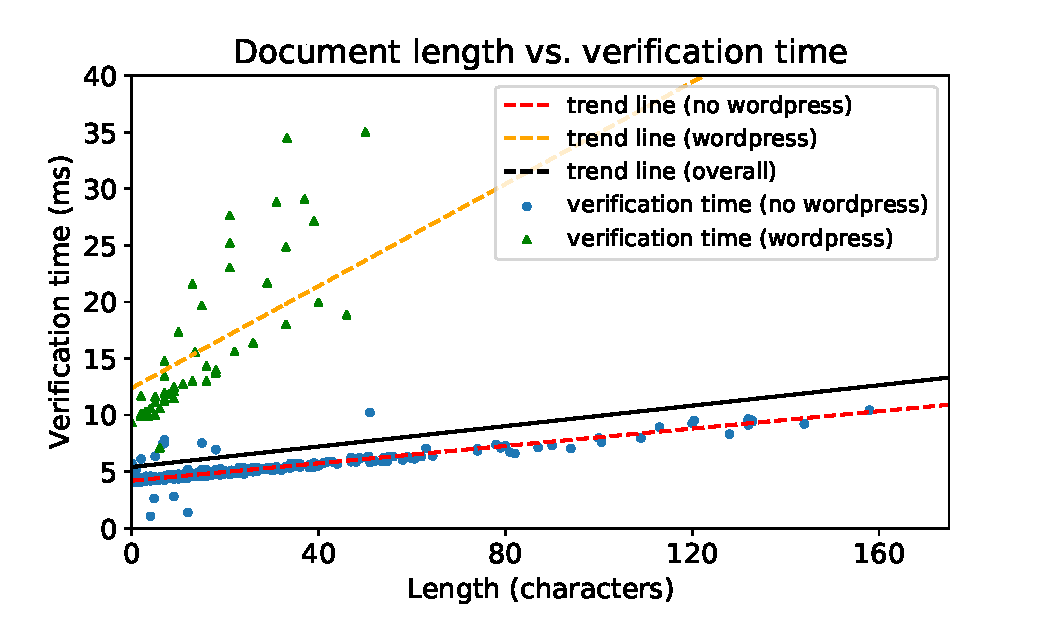
\includegraphics[scale=0.5]{results/string_length_vs_verification_time_small.pdf}
	\caption{Scatter plot of network filter time as a function of character length for top sites.}
	\label{fig:verification_time_string_length}
\end{figure}

 Figure ~\ref{fig:verification_time_string_length} shows the time spent by the call to our string verification function in the network filter as a function of the length of the string to be verified. The blue dots are the pages for which our framework probes tested negative, and the green triangles are the pages for which the probes tested positive: 55 in total. We applied least squares regression to calculate the shown trend lines. The Spearman's rank correlation values for no probe, probe, and overall are 0.91, 0.91, and 0.72 respectively, demonstrating positive correlation. Since both our probes and signatures use regex matching, we expect both trend lines to be linear, as seen in the graph. Recall that once a probe for a certain software passes, we perform a linear scan over the signatures for that specific software and check whether it applies to the given HTML string or not. Thus, we expect the slope of the line to be higher when a probe passes. Around 37.4\% of all web sites use frameworks covered by our probes~\cite{w3stats}, thus, we expect the impact of our network filter to be closer to the non-probe values, as corroborated by our overall trend line.

Additionally, for each website we recorded the number of loaded signatures. We report a 0\% FP rate for loaded signatures. Thus, we can infer with confidence that the rate of false positives for loaded signatures during an average user's web browsing is similarly low. This rate could possibly go up as the number of signatures and covered frameworks increases. It is likely that these websites are free of vulnerabilities covered by our signatures, as many of these websites are not running WordPress to begin with, and being the most popular, they would likely be updated quickly if a vulnerability is found; thus, the rate of FNs is likely extremely low as well.

\subsection{WordPress websites load times} \label{wordpress_sites}

We ran similar experiments as in Section 6.1, but with the WordPress sites described in Section 4.1. Thus, all of these have either one or multiple injection points in their HTML, and the network filter will spend an additional amount of time sanitizing these as defined by the signatures. Note that the data set is smaller here, and some of the trends might be harder to infer.

\autoref{fig:WordPress_slowdown} shows the results for slowdown with the extension running for these sites. Recall that the only difference between a page which passes the WordPress probe and one that matches a signature is that the latter has to replace a portion of the original string by its sanitized version. In this case we see a slowdown of less than 10\% for 60\% of sites, and less than 40\% for 96.25\% of them. The warm network filter curve suffers from a particularly high slowdown. We believe this to be the case because the locally hosted pages decrease the network component time, causing any overhead to be seen as relatively high. However, as 48\% of the original values were below 60ms, conclude a small impact on user experience as well.

\begin{figure}[h]
	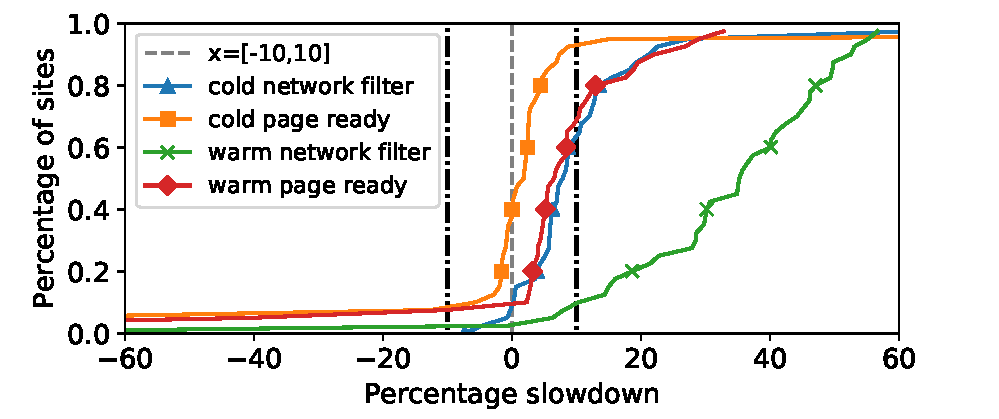
\includegraphics[scale=0.5]{results/extension_slowdown_wordpress_small.pdf}
	\caption{Cumulative distribution of relative percentage slowdown with extension installed for WordPress sites.}
	\label{fig:WordPress_slowdown}
\end{figure}

\iffalse
\autoref{fig:histogram_slowdown_wordpress} shows the probability density of the cold network filter slowdown. In this case, we see that the distribution is skewed more towards a higher slowdown. As it is harder to discern the trend for this data set than its top site counterpart, we have also plotted the normal distribution of the data between 3 standard deviations. 65\% of values are less than 10\%.

\begin{figure}[h]
	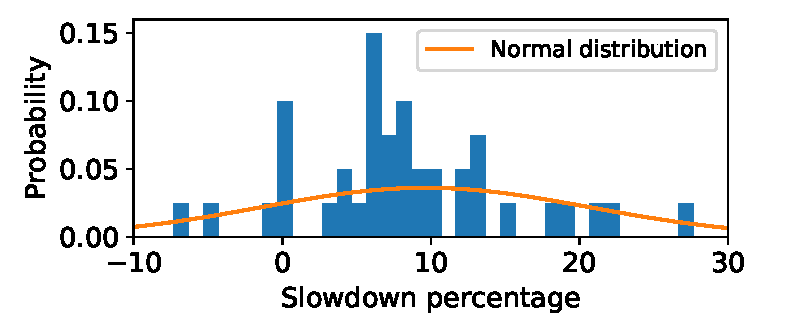
\includegraphics[scale=0.5]{results/density_histogram_filter_slowdown_wordpress_small.pdf}
	\caption{Density histogram of network filter slowdown for WordPress sites.}
	\label{fig:histogram_slowdown_wordpress}
\end{figure}
\fi

Finally, we report the string verification time as a function of its length, for the WordPress sites, shown in \autoref{fig:verification_time_string_length_wordpress}. The Spearman's rank correlation for this set of data is 0.630.


\begin{figure}[h]
	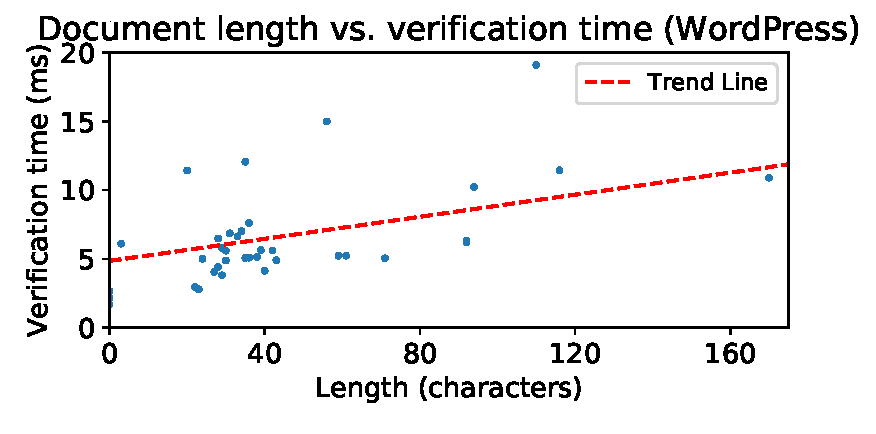
\includegraphics[scale=0.55]{results/string_length_vs_verification_time_wordpress_small.pdf}
	\caption{Scatter plot of network filter time as a function of character length for WordPress sites.}
	\label{fig:verification_time_string_length_wordpress}
\end{figure}
